\subsection{Medulloblastoma and pilocytic astrocytoma}
Pilocytic astrocytoma (PA) is a benign and slow-growing WHO grade I central nervous system (CNS) tumor.
PA is mostly characterized by piloid cells, Rosenthal fibers and eosinophilic granular bodies.
Often, compact fibrillar areas are next to loose microcystic areas.

Medulloblastoma (MB) is a malignant and fast-growing WHO grade IV CNS tumor.
MB is mostly characterized by small and densely packed cells with little cytoplasm.

PA and MB are shown next to normal brain tissue in \cref{fig:normal-pa-mb}.
See \citeauthor{Spies2023} \sidecite{Spies2023} for more on PA and MB characterization in HHG images.

\begin{figure*}
    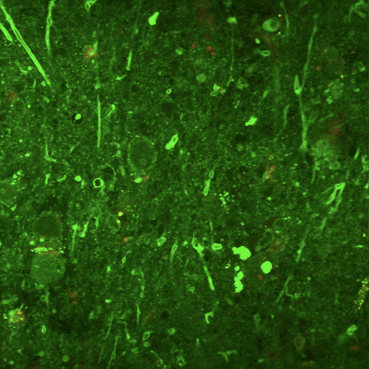
\includegraphics[width=0.3\linewidth]{pediatric-brain-tumours/images/normal.png}
    \includegraphics[width=0.3\linewidth]{pediatric-brain-tumours/images/pilo.png}
    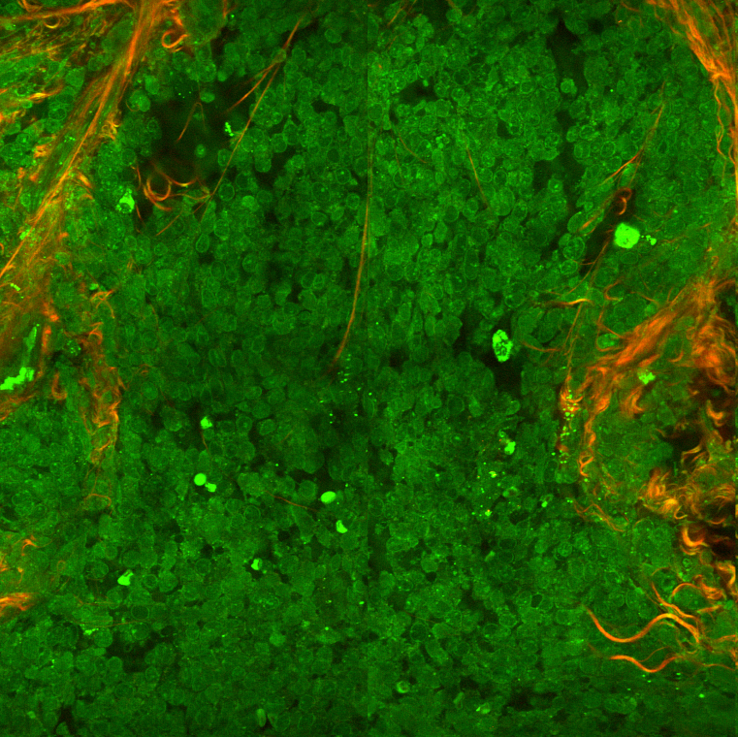
\includegraphics[width=0.3\linewidth]{pediatric-brain-tumours/images/medullo.png}
    \caption[Normal, pilocytic astrocytoma, and medulloblastoma HHG images.]{
        Higher harmonic generation images of normal (left), pilocytic astrocytoma (middle), and medulloblastoma (right) tissue.
        Normal brain tissue contains myelinated axons and neurons.
        Pilocytic astrocytoma is characterized by piloid cells.
        Medulloblastoma is characterized by high cellularity.
    }
    \label{fig:normal-pa-mb}
\end{figure*}
